%!TEX root = ../../csuthesis_main.tex
\chapter{绪论}



\section{研究背景}

随着人工智能、 计算机视觉,自动控制等技术极速发展,自动驾驶属于智能交通体系的关键部分,正由理论探究迈向商业化应用,自动驾驶系统一般包含感知,决策,控制这三个模块,而视觉感知处于信息获取的最前端,它的精准度和稳定性会直接影响到整个系统的安全性与智能水平,在繁杂的交通场景当中,精确地识别车辆,行人之类的动态物体,持续性地跟进它们,并及时判定这些目标的行为意图,这是做到安全行驶和路线规划的重要前提。

当下,依靠深度学习的目标检测和多目标跟踪算法在学术界和工业界被广泛性采纳,像 YOLO 系列,SORT/DeepSORT 这些颇具代表性的视觉跟踪算法已经具备了比较高的即时性和鲁棒性,但是在实际的交通场景当中,仅仅凭借跟踪得来的信息通常无法满足高级驾驶辅助功能(ADAS)的需求,系统不但要知道“是什么”和“在哪里”,而且还要明白“它打算做什么”,也就是针对前方目标的运动趋向和行为目的作出恰当的判定,进而预先展开风险预估和决策干涉,这样一种依托时空轨迹以及速度信息实施意图识别的本领,会变成未来智能驾驶系统的一项关键能力。

另一方面,由于受到真实交通场景数据收集成本高且难以控制等因素限制,虚拟仿真平台对于智能驾驶算法研发而言非常关键,Carla作为目前最具代表性的自动驾驶开源仿真平台之一,它给予了极为逼真的三维城市交通场景以及全面的传感器模拟功能,给研究人员赋予了一个可以掌控并重现的试验场所,本项研究依靠Carla平台,构建一个能够运行的目标追踪和意图识别系统,达成从视觉感知到智能判定的整个过程的设计与完成,具备很大的研究价值和实际意义。

综上可得,针对面向自动驾驶的视觉目标跟踪与意图分析展开研究,可促使感知系统由“感知当下”朝着“预测未来”方向发展,而且有益于提升自动驾驶系统的安全多余能力并优化交通行为的合理性,本课题所取得的研究成果会给未来的多目标智能预测,复杂场景认知等方向赋予工程操作根基和技术参照,具备较好的应用前景。

\section{国内外研究现状}

\subsection{目标检测研究现状}

目标检测就是把图像或者视频里的目标从其他不关注的地方分离出来,判定有没有目标,如果有还要找出它们所在的位置并识别出目标类别,这属于计算机视觉范畴内的一项任务,按照是不是用了深度学习作为界限,可以把目标检测算法分成传统目标检测算法和依靠深度学习的目标检测算法,传统目标检测算法要靠手工设计特征算子,采取先获取特征再做分类器这样的模式来达成目的。Viola和Jones提出了Viola-Jones人脸检测器 \cite{viola2001rapid},这个检测器运用Haar - like特征获取算子,借助AdaBoost分类器执行分类,而且采用由许多个分类器合成的Cascade级联分类器去提升识别率。Navneet Dalal等人\cite{dalal2005histograms}提出方向梯度直方图(Histogram of Oriented Gradients,HOG),它属于目标检测中的一种特征描述算子,该方法通过计算图像里局部区域梯度的方向来获取图像浅层的外观特征,不过HOG过于依赖局部梯度信息,所以其在复杂场景下的特征获取能力比较差。Felzenszwalb等人\cite{felzenszwalb2009object}以HOG为基础,提出了可变形组件模组(Deformable Part Model,DPM),DPM采取多组件策略,把目标拆解成许多部分之后再执行建模,从而使得DPM针对目标形变具备较强的鲁棒性。 传统目标检测算法大多依靠人工设定的特征获取算子去执行图像特征获取任务,当处于多尺度,密集型目标,极端天气等复杂环境的时候,其鲁棒性和准确率都会大幅下降,而且利用滑动窗口逐个计算图像特征的做法,还致使算法计算复杂度偏高,所以传统目标检测法无法符合即时检测的需求,很难在实际工业生产过程中加以运用。

深度学习快速发展之际,目标检测领域的研究收获了冲破性的进程,同传统目标检测算法比起来,依靠深度学习的目标检测模型历经海量图像数据的训练之后,可以“学会”怎样获取目标特征,当遭遇不同大小的目标以及复杂场景的时候,有着更强的鲁棒性和泛化性能,按照是否须要产生候选区域来分,凭借深度学习的目标检测算法可被划归为单阶段(one - stage)和两阶段(two - stage),两阶段的目标检测算法大致上分成两步,第一步选出图片里也许会存在物体的候选区域,第二步针对这些候选区域执行特征方面的分类和回归操作。Ross Girshick等人\cite{girshick2014rich}提出R-CNN目标检测算法,首先对输入图像使用选择搜索\cite{uijlings2013selective}(selective search)网络得到大概2000个不一样大小的候选区域,然后把所有候选区域统一缩放,变成227×227大小。 接着用CNN网络对全部候选区域执行特征获取,从而得到维度为2000×4096的特征向量,之后利用SVM分类器实施分类,并依靠回归器调节边界框的位置,R-CNN目标检测算法需针对大概2000个候选框逐个做特征获取,而且候选框之间会有不少重合部分,具备相同特征,这样便产生诸多多余操作,极大地影响到检测速度。为解决此问题,Ross Girshick等人\cite{girshick2015fast}又提出了Fast R-CNN,Fast R-CNN先把输入图片执行卷积,以得到相应的特征图。 之后把预先处理好的区域候选框投射到特征图上,这样做只需执行一次卷积运算,从而削减诸多不必要的卷积计算量,不同于R - CNN的分类任务 + 回归任务模式,FastR - CNN把这两个任务合并进同一个网络当中,不必再单独训练分类器和回归器,不过FastR - CNN算法仍然保留利用选择搜索算法来得到候选区域的做法,这个过程既耗费时间又很可能会忽略掉包含目标的区域。因此Shaoqing Ren等人\cite{ren2015faster}又提出了Faster R-CNN,此算法通过区域建议网络(RegionProposalNetworks,RPN)去获取区域候选框,达成了产生候选区域步骤同目标检测任务的融合。 FasterR - CNN算法中同时也提出了锚框(Anchor)这一关键思想,所谓锚框就是预先在图像上指定许多组大小比例不一的参照框,以此来尽量涵盖物体可能出现的位置。He Kaiming\cite{he2017mask}等人在Faster R-CNN的根基之上又提出了MaskR - CNN,这个算法用ROIAlign去替代FasterR - CNN里的ROIPooling,ROIAlign可把任意大小感兴趣区域的特征图划分成固定大小的小特征图,而且利用双线性插值取代了ROIPooling里的直接取整做法,从而化解了ROIPooling由于两次量化而产生的区域不契合(mis - alignment)现象。 在目标检测任务当中,利用IOU阈值去区分正负样本,如果IOU阈值更大一些,那么正样本的数量就会更少,相反如果减小IOU阈值,则会学到许多无关紧要的特征。Cai等人\cite{cai2018cascade}为了解决上述问题,提出了Cascade R-CNN,该算法采用级联式的结构,通过对多个感知器使用递增的IOU阈值进行训练,来解决因提高IOU阈值所引起的模型过拟合问题。

\subsection{目标跟踪研究现状}

多目标跟踪算法可分成依靠检测跟踪(TrackingbyDetection,TBD)和联合检测跟踪(JointDetectingTracking,JDT)这两种形式,TBD目标跟踪算法就是先通过目标检测算法得出含有物体的边界框,然后获取目标的运动信息,外观信息等等,最后用数据关联算法去计算目标之间的亲合力并执行目标关联。Bewley等人\cite{bewley2016simple}提出了 SORT 算法,它属于经典的依靠检测的目标跟踪算法,该算法把Faster R - CNN当作检测器,利用卡尔曼滤波来预估并更新物体的运动特征信息,通过匈牙利算法实施数据关联,而且用IOU当作度量标准以创建联系,这样就能做到对多个目标的跟踪。Wojke 等人\cite{wojke2017simple}提出了 DeepSORT 多目标跟踪算法,此算法在SORT的基础上添加级联匹配,用卷积神经网络得到目标外观特征,从而削减面对遮挡时出现的身份切换状况。Yu 等人\cite{yu2016poi}提出了 POI 算法,采用 Faster R-CNN 作为检测器,并使用 skip pooling 和 multi-region 两种策略来提高检测精度,利用改进的 GoogLeNet\cite{szegedy2015going}网络进行特征提取。Sun 等人\cite{sun2019deep}提出了深度亲和网络(DAN),DAN 网络以端到端的方式对目标物体的外观特征进行学习,通过物体和环境的分层特征计算出在不同帧中目标之间的亲和度。Chen 等人\cite{chen2018real}将检测和跟踪结果组成一对候选框,提出了一种得分函数用于衡量每一对候选框的匹配程度,使用非极大值抑制算法依据得分情况进行筛选。Zhang 等人\cite{zhang2021fairmot}把目标检测和特征获取融合进同一个网络里做,先利用编码器 - 解码器结构得到图像特征,分流之后,用两个分支各自做边界框预测和目标外观特征获取,再通过预测目标中心点处的特征实施边界框的时序结合。Liang 等人\cite{liang2022rethinking}提出 CSTrack 算法,采用 CCN(交叉相关网络)来改进检测与重识别间的协作学习。将目标检测和外观特征提取进行解耦,通过使用自注意力的方式获得自注意力权重图和交叉相关性权重图,并利用 SAAN\cite{zhao2020saan}(尺度感知注意力网络)对特征提取网络进行优化。Liang 等人\cite{liang2022fake}在 CSTrack 的基础上引入时间信息来修正检测器结果,并提出了重检测网络来重新加载被错误分类的目标。Yu 等人\cite{yu2022relationtrack}提出了 GCD(Global Context Disentangling)模块,该模块能将特征图解耦成检测特征和重识别特征两部分,同时采用可变形注意力机制来学习目标和环境之间的关系。

联合检测跟踪算法是将检测任务与跟踪任务进行合并,仅使用一个网络来实现多目标跟踪任务。Peng 等人\cite{peng2020chained}提出了一种 CTracker 算法,该算法首次将目标检测、特征提取、数据关联三个模块集成到单个网络中,实现了端到端的联合检测跟踪。同时还设计了一种联合注意力模块(JAM,Joint Attention Module)来突出检测框中的有效信息区域。Xu 等人\cite{xu2020deep}提出了 DHN(深度匈牙利算法),以可微的方式对检测框和预测框进行匹配,以及提出了一种新的损失函数用于训练联合检测跟踪范式的多目标跟踪器。Pang 等人\cite{pang2021quasidense}提出 QDTrack 算法,通过采用多个正负样本同时计算损失的方式来对特征提取网络进行训练,是一种只利用 ReID 特征而不需要位置和运动信息的多目标跟踪方法。Zhou 等人\cite{zhou2020tracking}提出了 CenterTrack 算法,使用 CenterNet\cite{zhou2019objects}目标检测算法来对目标中心进行定位,CenterTrack 依据上一帧的检测结果得到热量图,峰值代表目标中心点,并采用高斯渲染的方法进行模糊处理。模型利用两个额外的并行分支来预测当前目标相对于上一帧时的水平和竖直方向偏移量。Wu 等人\cite{wu2021track}提出在线多目标联合检测追踪模型,该模型先通过CenterNet得到图像特征,再凭借CVA模块算出两帧图像里目标的偏移量,从而得到目标间的关联情况,之后利用MFW模块去传播并加强目标特征,最后依靠头部网络把传播过来的特征和当前特征加以处理,以此做到检测和追踪。Wang 等人\cite{wang2021multiple}提出了 CorrTracker 算法,利用局部相关模块来构建目标与周围环境之间的拓扑关系,从而加强模型在密集场景中的识别能力。Sun 等人\cite{sun2020transtrack}提出 TransTrack 算法,该算法采用 transformer\cite{vaswani2017attention}架构,利用 Query-Key 机制来跟踪当前帧中已存在的目标以及对新目标进行检测。通过在一次拍摄中完成目标检测和目标关联,建立了一种新的联合检测跟踪范式。Chu 等人\cite{chu2023transmot}提出了 STGT 模型,通过将追踪目标轨迹视作稀疏赋权图来构建目标间的空间关系。STGT 构建了一个空间图 transformer 编码器、时间 transformer 编码器和一个空间 transformer 解码器。利用稀疏图来提升训练和推理时的计算速度。并且由于获取了目标间的结构信息,因此比一般的 transformer 也更加有效。

\subsection{意图分析研究现状}

最早关于识别驾驶意图的讨论可以追溯到 Andrew 等人的一项研究\cite{liu1997realtime},他们感到能够通过剖析驾驶员的行为动作去预估其意图,在该项研究当中仅仅利用了车辆的动态数据,譬如横摆角,横摆角速度以及车速等来判定驾驶员有无转弯或者变换车道的意图,若想对周边车辆的变换车道意图实施识别,则须要综合运用感知,数据融合,数据处理等诸多技术\cite{zhang2023highway}。感知和数据融合技术会把全部从传感设备传送过来的信号加以融合,从而产生出周边所有交通情况以及其它环境因素的相关信息,智能车辆会把这些信息从自己的车辆坐标系转变成目标车辆的坐标系,并进一步处理成可供识别算法采用的特征变量,所以除了识别方法之外,特征变量的选取对于识别效果而言同样十分关键,就单个目标车辆来说,当前被广泛性采纳的信号涵盖纵向/横向位置,速度和加速度\cite{woo2017lane}。主车的意图识别可以通过车内传感器获得大量有效信息,比如方向盘和制动/油门踏板信号,甚至驾驶员本身的状态等。然而,在车联网技术尚未成熟的当下,目标车辆内的这些信息难以获取。Zhang 等\cite{zhang2018lane}使用目标车辆及其四辆邻近交通车辆的信息,包括它们之间的相对速度和距离,来预测换道行为。Leonhardt 等\cite{leonhardt2017feature}也采用了类似的特征变量来研究换道预测。部分研究使用了目标车辆周围的更多相邻车辆以及与每个相邻车辆相关的更多信息(比如状态量的历史记录)\cite{patel2018predicting}。Altch 等\cite{altche2017lstm}甚至考虑了九辆车来提高预测性能。

2016 年,日产研制出了前沿科技 ProPILOT,其安装的实力强劲的摄像机可以较为容易的检测出车相对道路的偏离距离\cite{zhang2016nissan}。雪铁龙LDWS系统装有6个电子传感器,当汽车经过车道标记线时,由于光线反射不同,检测单元就会把信息传送到车载控制中心,车内自带的振动马达便会向驾驶员发出警报,该系统价格便宜,适应能力较好,但在复杂电子环境中的表现不佳,元件精准度有所下降,现在只有C5,C6车型才配备此系统。Google也投入了相应研发工作,凭借高效能的软件及智能探测装置,并融合雷达与摄像技术之后,就能在各种复杂状况之下全方位探测周边环境\cite{wang2020autonomous},其结合 GPS 技术的车道偏离技术可以及时矫正汽车的行驶轨迹,并且误差可以达到厘米级。Enache 等\cite{enache2009driver}提出了新的计算方法,通过预瞄偏差及车辆方向偏差综合信息来估计车路之间的相对距离;Cualain 等\cite{cualain2012automotive}利用卡尔曼滤波和霍夫变换建立了车道边界的模型,计算车辆本身的参数及建立新的预警规范来设计预警系统的阈值;Mammar 等\cite{mammar2006time}通过计算道路曲率、方向偏差等估计车辆跨过车道线的时间;Ulsoy 等\cite{chiu1996time}利用准确度较高的算法估计TLC 的不确定,考虑到了不同方面的误差;Gaikwad 等\cite{gaikwad2015lane}通过对感兴趣区域的划分,建立实际车道偏离的度量标准。

\section{研究目标与内容}

本课题意在设计并完成一套依靠视觉感知的自动驾驶目标跟随及意图分析体系,利用Carla仿真平台创建起可控制的交通环境,通过整合深度学习目标跟随算法和凭借物理信息的行为推断机制,达成对诸如车辆,行人之类的动态交通目标持续不断地辨别,路线跟随以及运动意图判别,而且可以在图形界面上即时显现跟随进程和意图分析成果,进而给智能驾驭体系给予基本的感知支持。

为实现上述目标,本课题主要围绕以下几个方面开展具体研究与开发工作:

\textbf{数据集构建与处理。}在 Carla 提供的仿真场景中,安排好本车并自动生成车流,利用安装的RGB摄像头针对周边交通目标展开图像收集和注解工作,获取含有图像帧,目标边框,目标速度等信息的初始数据,从而创建起供视觉分析用的多模态数据集,还要规划出合适于后续分析和训练的标注形式以及存储架构。

\textbf{视觉目标跟踪模型设计与集成。}本系统把依靠深度外观特征加强DeepSORT算法当作目标跟踪模型,通过对视频帧里的检测结果执行轨迹层面的数据关联,达成对车辆和行人的单独身份标识以及跨帧追踪,系统允许在单目标跟踪模式时自动挑选“最为靠近本车”的目标实施连续跟踪,而且会把跟踪成果即时绘制到屏幕图像上。

\textbf{基于速度信息的意图分析方法设计。}在目标跟踪的基础上,提取目标在世界坐标系下的运动方向与速度大小,并结合其与本车的相对位置关系,设计运动意图识别规则体系。采用物理特征量(如点积关系、欧氏距离变化、速度阈值)判断目标是否存在“靠近”“远离”“危险靠近”等行为状态,并输出中文提示文本以实现可视化展示与预警反馈。

\textbf{系统集成与仿真测试。}将上述模块集成为一个完整的自动驾驶视觉分析系统,结合 Carla 提供的控制接口与传感器 API 实现全过程联动,在 Town10 与 Town01 两个典型城市街景场景中分别进行系统测试与功能验证,评估模型在不同场景下的运行效率与判断准确率,并结合帧率等性能指标进行可行性分析。

本研究着眼于自动驾驶核心任务需求,通过仿真数据收集,视觉追踪,行为分析以及即时显示这四个方面展开工作,塑造起由感知至判断的完备流程,具有较大的应用价值和操作意义。

\section{本文结构框架}

本课题以自动驾驶场景中的视觉感知和行为预测作为核心内容,凭借Carla仿真平台所营造出的高真实度交通环境以及Python接口功能,利用模块化设计理念构建起“数据采集—目标跟踪—意图分析—可视化表现”这样一条连贯的工作流,并创建出一个能够实际运作且具备拓展性的目标感知与行为识别系统,整个研究手段包含数据采集与前期处理,目标跟踪算法设计,意图分析部分开发,可视化体现及系统整合这四个重要步骤,其大致流程可由下图表示出来:

\begin{figure}[H]
	\centering
	\makebox[\textwidth]{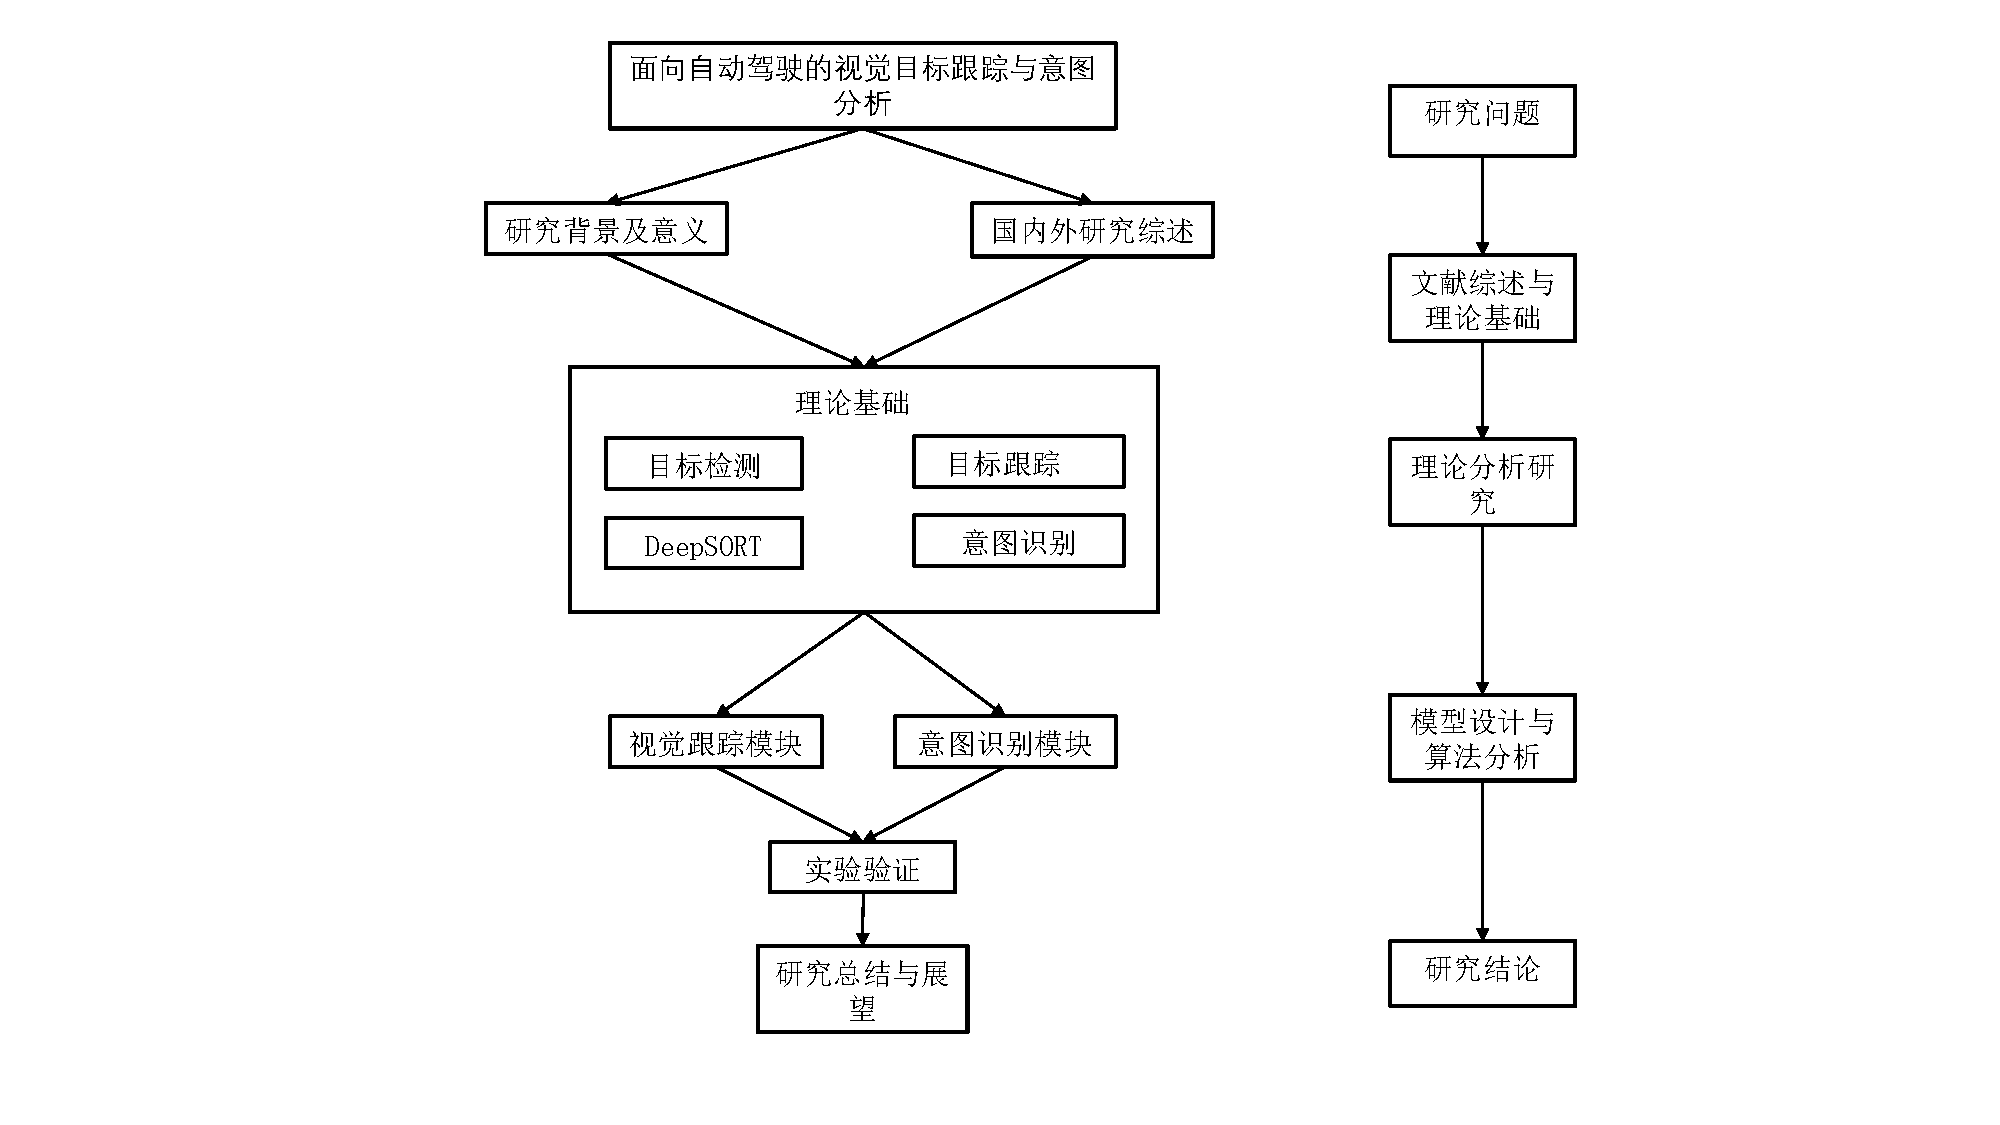
\includegraphics[width=1.2\textwidth]{images/图1 系统技术路线图.pdf}}
	\caption{论文结构框架图}
	\label{fig:example_image}
\end{figure}


在数据采集方面,系统借助Carla平台产生典型交通场景,优先选用Town10和Town01当作试验场所,在车上装配前向RGB摄像头来收集图像数据,每一幅图像经过处理之后,可以得到车辆的二维边框,目标ID,速度大小这些结构化的数据。为了便于后面的训练和分析,系统在运行的时候会自行保留图像帧(.jpg格式)以及对应的标注文件(.json格式),其中涵盖边框坐标,目标速度,是不是当前正在追踪的对象等重要信息,从而创建起带有时间顺序特点的感知数据集,保证其具有重现性和可拓展性。

目标跟随时系统的关键所在,本设计融合了 DeepSORT 跟踪算法,该算法把外观特征获取同卡尔曼滤波融合起来,既维持住即时性又保有不错的数据关联水准,通过调用 CarlaAPI,可以马上得到当前场景里全部车辆的三维坐标位置,再加上来自前端图片当中的二维边框信息,就可以做到让目标在图像空间持续被标记出来,为使算法一直关注当下对本车最具潜在交互危险的那个对象,采取“先近后远”的挑选原则来决定要跟踪哪个目标,而且每次只盯住单独一个即可,这样做既能削减运算量又能精简意图分析的复杂程度。

在行为识别上,系统依靠目标的速度向量,方向角度及其相对于本车的位置,形成起轻量级的意图分析模块。这个模块通过计算目标车辆速度方向与本车的点积关系,融合速度大小和空间距离的动态改变状况,来判定目标的当下行为趋向,其中涵盖“靠近中”“远离中”“危险靠近”“目标稳定”等状态,而且利用阈值合成判断实施分级判断,在实际运作过程中,系统能够及时预测目标行为,并把分析成果用中文文本形式显示在跟踪框上面,从而提升系统的人机交互性和直观程度。

整个系统的主控逻辑存在于Carla的同步刷新机制当中,通过game\_loop()主循环来达成数据获取,图像渲染,目标识别,意图计算以及结果显示等全过程的联动,系统利用Pygame实施图像渲染和键盘交互,允许用户对本车行驶执行手动操控,而且会自动保存图像和标签,有益于后续的模型训练和性能考量,总体架构很好地表现出模块化,可检测和可拓展的设计理念,可以有效地支撑不同场景之下的视觉感知和行为分析研究,具备较好的工程化实现根基。




\begin{tabular}{l l}
%  \verb|\songti| & {\songti 宋体} \\
%  \verb|\heiti| & {\heiti 黑体} \\
%   \verb|\kaiti| & {\kaiti 楷体}
\end{tabular}
